\documentclass{article}


\usepackage[margin=0.6in]{geometry}
\usepackage{amssymb, amsmath, amsfonts}
\usepackage{tabularx}
\usepackage{arydshln}
\usepackage{mathtools}
\usepackage{changepage}
\usepackage{asymptote}
\usepackage{cancel}
\usepackage{physics}
\usepackage{pgf}
\usepackage{enumerate}
\usepackage{placeins}
\usepackage{nth}
\usepackage{array}
\usepackage{tikz}
\usetikzlibrary{arrows,automata}
\tikzset{
  saveuse path/.code 2 args={
    \pgfkeysalso{#1/.style={insert path={#2}}}%
    \global\expandafter\let\csname pgfk@\pgfkeyscurrentpath/.@cmd\expandafter\endcsname
      % not optimal as it is now global through out the document
                           \csname pgfk@\pgfkeyscurrentpath/.@cmd\endcsname
    \pgfkeysalso{#1}},
  /pgf/math set seed/.code=\pgfmathsetseed{#1}}
\usepackage{nicefrac}
\usepackage{pgfplots}
\usepgfplotslibrary{polar}
\pgfplotsset{holdot/.style={fill=white,only marks,mark=*}}
\pgfplotsset{soldot/.style={only marks,mark=*}}
\newcommand{\enth}{$n$th}
\newcommand{\Rl}{\mathbb{R}}
\newcommand{\Cx}{\mathbb{C}}
\newcommand{\sgn}[1]{\text{sgn}\qty[#1]}
\newcommand{\ran}[1]{\text{ran}\qty[#1]}
\newcommand{\E}{\varepsilon}
\newcommand{\qiq}{\qquad \implies \qquad}
\newcommand{\half}{\nicefrac{1}{2}}
\newcommand{\third}{\nicefrac{1}{3}}
\newcommand{\quarter}{\nicefrac{1}{4}}
\newcommand{\f}[3]{#1\ :\ #2 \rightarrow #3}
\newcommand{\Dx}{\Delta x}
\newcommand{\Dy}{\Delta y}
\newcommand{\Dt}{\Delta t}
\newcommand{\hot}{\text{h.o.t.}}
\newcommand{\centdiff}{\frac{u_j^{n+1} - u_j^n}{\Dt}}

\newcommand{\tridsym}[3]{
    \qty(\begin{array}{ccccc}
                    #1 & #2 & & & \\
                    #3 & #1 & #2 & & \\
                    & \ddots & \ddots & \ddots &  \\
                    & & #3 & #1 & #2 \\
                    & & & #3 & #1
                \end{array})
}


\DeclareMathOperator*{\esssup}{\text{ess~sup}}

\title{MAT 228B Notes}
\author{Sam Fleischer}
\date{February 17, 2017}

\begin{document}
    \maketitle

    \section{Non-Rectangular Domains}
        How do we solve $u_t = \laplacian u$ on a non-rectangular domain?  There are three ways:
        \begin{enumerate}[\ \ (a)]
            \item Cartesian mesh (embed the shape in a rectangle, mesh the rectangle).  The question is what to do at the points near the boundary.
            \item Body-fitted mesh (warped rectangle.. conformal mapping).  The question is how to transform to another coordinate system.  And, what happens to the PDE after the coordinate transform?
            \item Unstructured mesh (throw down points on the interior and triangulate somehow with points on the boundary).  The question is which points are ``next to'' which points.  This method is used with finite element methods (not finite difference (volume) or spectral)
        \end{enumerate}

        \subsection{Cartesian Grid}
            \begin{figure}[ht!]
                \centering
                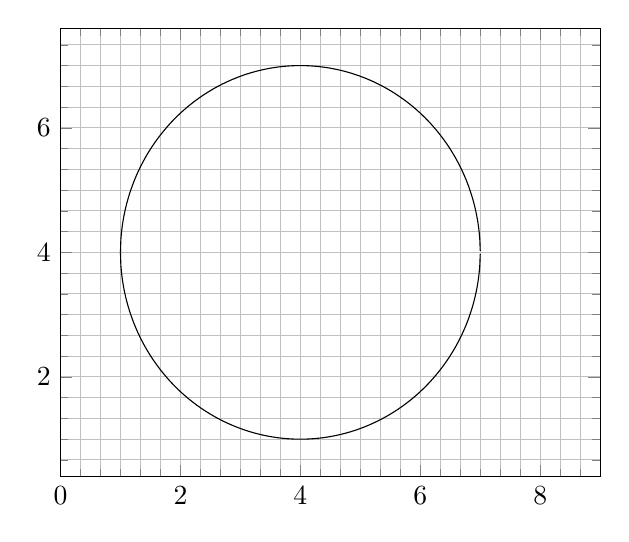
\begin{tikzpicture}
                    \begin{axis}[smooth,samples=1000,minor tick num=5,grid=both,xmin=0,xmax=9]
                        \addplot[domain=1:7] {(9 - (x-4)^2)^0.5 + 4};
                        \addplot[domain=1:7] {-(9 - (x-4)^2)^0.5 + 4};
                    \end{axis}
                \end{tikzpicture}\hfill
                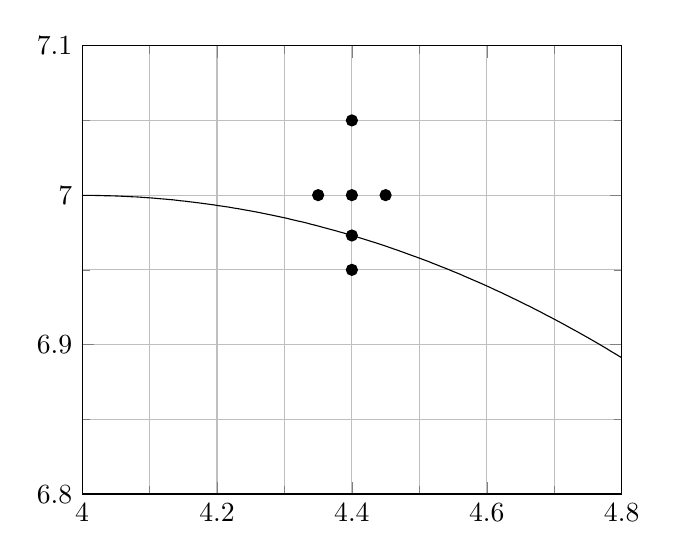
\begin{tikzpicture}
                    \begin{axis}[smooth,samples=1000,minor tick num=1,grid=both,xmin=4,xmax=4.8,ymin=6.8,ymax=7.1]
                        \addplot[domain=1:7] {(9 - (x-4)^2)^0.5 + 4};
                        \addplot[domain=1:7] {-(9 - (x-4)^2)^0.5 + 4};
                        \addplot[soldot] coordinates{(4.4,7)(4.4,7.05)(4.4,6.95)(4.35,7)(4.45,7)(4.4,6.973)};
                    \end{axis}
                \end{tikzpicture}
            \end{figure}
            For a point near the grid.  Suppose $P$ is a point where the points to the east $E$, west $W$, and north $N$ are still in the domain, but the point to the south $S$ is outside the domain.  Call $B$ the boundary point between $P$ and $S$.  So $\laplacian = \partial_{xx} + \partial_{yy}$ where $\partial_{xx}$ is unchanged, but we need to modify the discretization of $\partial_{yy}$.  There are two ways to do this:
            \begin{enumerate}[\ \ (a)]
                \item We can add an equation at point $S$ to extrapolate a value from inside.
                \item Or, we could exclude $S$ by modifying the stencil of $P$.  Rather than $N$, $E$, $S$, and $W$, use $N$, $E$, $B$, and $W$.  So, $y_P - y_B = \alpha \Dx$ for $\alpha \in (0,1)$, so $$u_{yy}(P) \approx \frac{2\alpha u_N - 2(\alpha + 1)u_P + 2u_B}{\alpha(\alpha + 1)\Dx^2}.$$  This is first-order accurate.
            \end{enumerate}
            The heat equation (or related equations) we have $\order{\Dx}$ truncation errors, but the solution will be $\order{\Dx^2}$.  In 1D, for the Poisson equation, an interior point $\order{\Dx} = \tau$, but $\order{\Dx^2}$ error.  The boundary point $\order{1}$ but still get $\order{\Dx^2}$ error.

            You could also put a finer mesh inside parts of a coarser mesh, but there are problems at the ``coarse-fine interface.''

        \subsection{Boundary-Fitted Meshes}
            We need a transformation from a rectangle to the physical domain.  So we'll call the original domain $\vec{x} = (x,y)$ and the rectangle is $\vec{\xi} = (\xi,\eta)$.  So we want a mapping $\vec{x} = \vec{F}(\vec{\xi})$.  Just mesh on $\vec{\xi}$.

            Example: Let's solve on an annulus in 2D.
            \begin{itemize}
                \item Use polar coordinates.  So $r \in (a,b)$ and $\theta \in (0,2\pi)$.  So $x = r\cos(\theta)$ and $y = r\sin(\theta)$.
                \begin{figure}
                    \centering
                    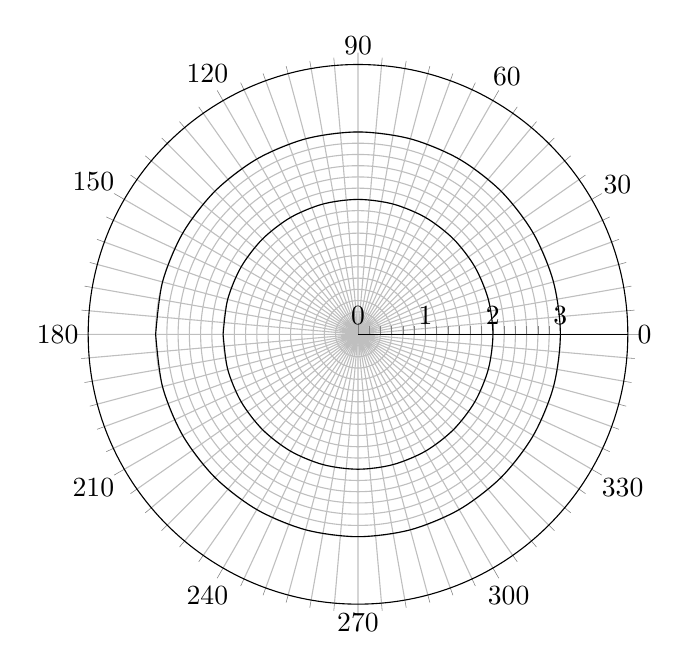
\begin{tikzpicture}
                        \begin{polaraxis}[smooth,ymax=4,ytick={0,1,2,3},minor tick num=5,grid=both]
                            \addplot[domain=-180:180] {2};
                            \addplot[domain=-180:180] {3};
                        \end{polaraxis}
                    \end{tikzpicture}\hfill
                    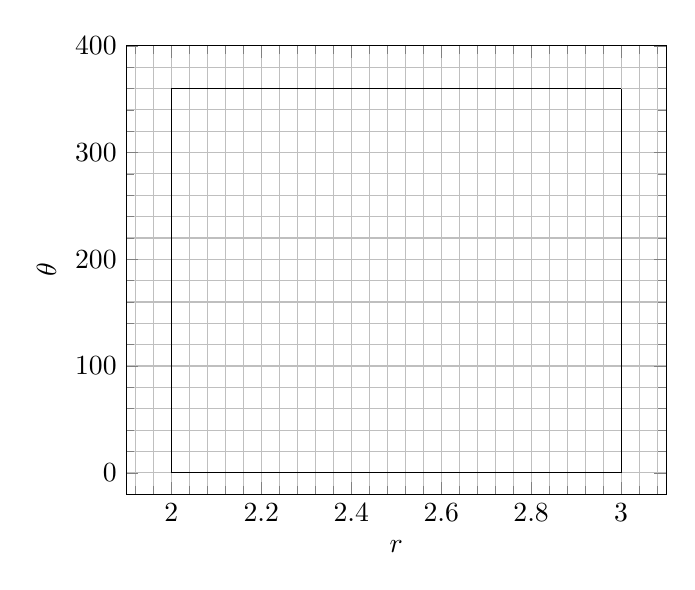
\begin{tikzpicture}
                        \begin{axis}[smooth,xlabel=$r$,ylabel=$\theta$,xmin=1.9,xmax=3.1,ymin=-20,ymax=400,grid=both,minor tick num=4]
                            \addplot[domain=2:3] {0};
                            \addplot[domain=2:3] {360};
                            \draw (axis cs:2,0) -- (axis cs:2,360);
                            \draw (axis cs:3,0) -- (axis cs:3,360);
                        \end{axis}
                    \end{tikzpicture}
                \end{figure}
                \item We get $\laplacian u = \frac{1}{r}\frac{\partial}{\partial r}\qty(r\frac{\partial u}{\partial r}) + \frac{1}{r^2}\frac{\partial^2 u}{\partial \theta^2}$ in polar coordinates.
            \end{itemize}
            For  non-polar coordinates, we have $\vec{x} = \vec{F}(\vec{\xi})$.  We want a mesh in $\vec{\xi}$ space.  So, define
            \begin{align}
                J_{ij} = \frac{\partial \vec{F}_i}{\partial \vec{\xi}_j}
            \end{align}
            and $g = J^TJ$, with $\abs{g} = \text{det}(g)$.  Then we get
            \begin{align}
                \laplacian u = \sum_{i,j}\frac{1}{\sqrt{\abs{g}}}\frac{\partial}{\partial \vec{\xi}_j}\qty(\sqrt{\abs{g}}g_{ij}^{-1}\frac{\partial}{\partial\vec{\xi}_j}u)
            \end{align}

\end{document}












